\chapter{Experiment Design}
\label{chapter:studysetting_conduction}
This master's thesis proposes an experiment that answers the research question RQ1: How does the visual perspective on a virtual gidance visualisation influence Motor Learning in Virtual Reality. This chapter describes the design of the experiment. First, the independet variables, namely the VPs, are determined in section~\ref{sec:visualPerspecticves}. Afterwards, the task for the experiment is developed in section~\ref{sec:taskDesign}. Finally, section~\ref{sec:measures} describes the independent vairables of the experiment.

\section{Visual Perspectives}
\label{sec:visualPerspecticves}
The last chapter pointed out five visual perspectives, compare figure~\ref{fig:perspectives}. All VPs are worth investigating, and a comparative study with all five visual perspectives is desirable. However, to reduce complexity and the number of participants\footnote{Due to COVID-19 pandemic}, this work will focus on three visual perspectives.\\
Figure~\ref{fig:perspectives} shows three main classes of VPs: ego-centric, exo-centric and perspectives which contain both. To answer the research question, it is indispensably to examine at least one of each class. The ego-centric VP is the only VP in the g-class and though chosen by default. The exo-centric VP can be realised as purely exo-centric or augmented exo-centric. The combination of ego-centric and exo-centric can be realised as ego \& exo-centric or ego \& augmented exo-centric. However, before the exo-centric VP and the combination can be chosen, a closer look at the mechanics that makes Motor Learning in VR possible is necessary.

\subsection{Excursion: Mechanics for Motor Learning in Virtual Reality}
For teaching movements in Virtual Reality in the exo-centric VP, the following issue arises: the GV can move out of the learner's field of view by the movement itself. Szenario: the learner and the GV stand side-by-side. The learner sees the GV to the left. The GV now indicates a movement to turn by 90 degrees to the right. As soon as the learner follows this movement, the GV will move out the field of view of the learner. After the movement ended, th GV is located behind the learner. The learner cannot see a GV standing behind the learner.\\
This issue is solved in existing work with either the restriction of movements~\cite{freethrowsimulator,elearningma} or multiple representations of the GV around the learner~\cite{thaichichua,mythaichicoaches}. The restriction of movements has a strong influence on the task design and is therefore not desirable for the study proposed in this master's thesis. Consequentially, for exo-centric visual perspectives, multiple representations for the GVs on strategic positions around the learner are necessary.\\

In the ego-centric VP, another issue arises during the teaching of locomotion movements. To understand this issue, two aspects have to be clear before. (1) The nature of an ego-centric GV is to be located inside the learner at any time. (2) A GV indicates movements by moving itself. If the GV is about to indicate a movement away from the learner, the GV is moving out of the student's body. However, a GV that is outside of the learner's body is no longer ego-centric.\\
A possible solution is given by the centricity continuum by Wang and Milgram~\ref{fig:ego-exo-continuum}. Following the centricity continuum's nature, the tethering distance can be increased by a small amount, and the visual perspective can still be classified as ego-centric. But now arises the question of how far the tethering distance can be increased, with which the perspective still feels ego-centric, but the indication of the movement is considerable. For simplicity, this distance is further called ego-centric tethering distance (ETD). To determine a reasonable ETD, an informal formative test\footnote{A formal study with more participants was not possible because of the COVID-19 pandemic. This holds for all upcoming formative tests.} was conducted with one participant. The participant was a former Computer Science Student with expertise in VR-systems, but had no prior knowledge about Motor Learning. During the formative test, the participant was asked to follow movements in the ego-centric visual perspective. The first movement was conducted with an ETD of 5cm. For the following movements, the ETD was increased by 5cm each. After each movement the participant was asked about the ability to follow the movements. The subjective assessment of the participant and my observations yielded best for an ETD between 15cm and 30cm. These two values are further called:
\begin{itemize}
	\item[] $ETD_{min}=15cm$
	\item[] $ETD_{max}=30cm$
\end{itemize}
Based on $ETD_{min}$ and $ETD_{max}$ the speed mechanic is developed. The speed mechanic controls the speed of the playback of the GV. At $ETD_{min}$ and below, the animation plays at normal speed. At $ETD_{max}$ the GV stops. Between $ETD_{min}$ and $ETD_{max}$ the animation speed of the GV is linearly interpolated, compare figure~\ref{fig:speed_mechanic}.
\begin{figure}[htb]
	\centering
	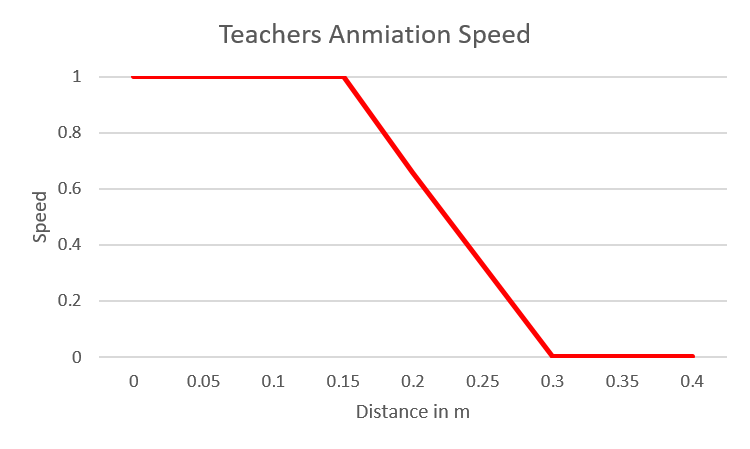
\includegraphics[width=0.6\textwidth]{figures/speed_mechanic_chart.png}
	\caption[speed mechanic chart]{speed mechanic chart}
	\label{fig:speed_mechanic}
\end{figure}
The speed-mechanic was evaluated by an informal formative test with one participant. The participant was a PhD student of Computer Science and had little experience with VR-systems, and none in Motor Learning. The participant's task was to follow the GV in the ego-centric visual perspective. Observations showed that the participant could follow the movement at ease. The opinion of the participant about the speed-mechanic was very positive ("It did not run away. I had no problem to follow the woman (ed: GV).").\\
With this short excursion, a reasonable decision for the exo-centric VP and the combination can be made.\\

In the ego-centric visual perspective, the learner sees the GV inside the own body. Here, the learner can see the relation of the own body to the GV directly. In the pure exo-centric visual perspective, this relation cannot be seen. Thereby, the position of the learner in relation to the GV must be guessed. That, in turn, makes the application of the speed-mechanic - which is necessary for ego-centric guidance - nearly impossible. A mechanic that is used in all conditions but one could lead to biased data, compare table~\ref{tab:mechanics}.
\begin{table}[htb]
	\centering
	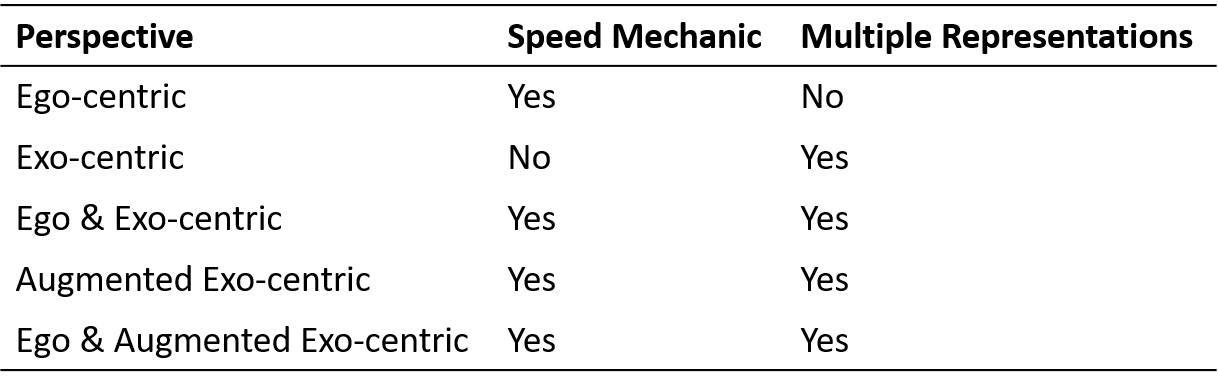
\includegraphics[width=0.6\textwidth]{figures/mechanics_comparison.png}
	\caption[Mechanics for Motor Learing in Virtual Reality]{Mechanics speed and multiple representations and in which VP they are applied.}
	\label{tab:mechanics}
\end{table}
The mechanic of multiple representations does not influence the study's validity because the mechanic would solve an issue that does not exist in the ego-centric perspectives. Furthermore, any VP with more than one representation is an exo-centric VP.\\
In the augmented exo-centric VP, a virtual copy of the learner is located inside the exo-centric GV. The copy lets the learner see the relation of the own body to the GV. Furthermore, augmenting the exo-centric GV with the learner is widely used and evaluated in related work~\cite{YouMove,thaichichua}. Consequently, the augmented exo-centric VP will serve as the exo-centric VP.\\
With the ego-centric and exo-centric VP set, the combination can be determined. In the ego-centric VP, the learner has a direct comparison of the own posture to the GV posture in the ego-centric VP. In the augmented exo-centric VP, the learner has a direct comparison of the own posture and the GV posture in the exo-centric VP. For a direct comparison of the own posture and the GVs posture in the ego-centric VP AND the exo-centric VP, the ego \& augmented exo-centric VP is chosen as the combination. The ego \& augmented exo-centric VP is the true combination of ego-centric and augmented exo-centric.\\
For simplification, the augmented exo-centric VP will be further called exo-centric VP, and the ego \& augmented exo-centric will be further called ego \& exo-centric VP.\\
The ego-centric VP, exo-centric VP and the ego \& exo-centric VP are the independent variables of the study and form the three study conditions EGO, EXO, EGO \& EXO.

\section{Task Design}
\label{sec:taskDesign}
Hornb\ae{}k~\cite{hornbaek} identified three main types of tasks in HCI studies: representative tasks, simple tasks and tasks that use task-specific hypothesis. RQ1 states that the main investigation field is Motor Learning. Motor Learning is strongly related to real-world movements. Evidently, the study task is a representative task.\\
Real-world tasks that include the handling of physical load can found in a wide range of activities. For example, a storekeepers job is to clear a palette of cardboard boxes. This task includes unloading the palette, scale the boxes, measure the dimensions of the boxes and finally store them in a rack. Another example is the work at a grinding machine. The worker takes a slug from a shelf and works on it until the slug becomes a workpiece. After that, the workpiece is carried to a measurement instrument to be verified. There are plenty of other examples, but these two already clarify that tasks which include the handling of physical load consist out of the elemental tasks for manual material handling: lift, lower, push, pull, hold.\\
The idea for the study task is to chain these elemental tasks together to create a Unit-Combined-MMH task that representatively stand for a wide range of tasks that includes the handling of physical load. To achieve this, several aspects have to be taken into consideration: (a) the artefacts with which the learner will interact, (b) a reasonable task decomposition into sub-tasks and their chaining that allows the investigation of sub-tasks. Furthermore, the experiment needs a (c) structure. (c) will reveal the necessity of three tasks. These tasks have to be (d) equally complex. This section will subsequently discuss (a-d) and propose the task for the study.

\subsection{(a) Artefacts}
A task that includes the handling of physical load obviously needs a physical load. In real-world tasks, the physical load can be everything a human can handle. The physical load for this task should fulfil the following criteria. First, the load should have a significant weight, that it is perceived as a load, but at the same time, any healthy person with no previous illnesses can handle it without getting injured. Secondly, the physical load should give enough freedom for interactions. A simple box fulfils the criteria and has a relation to physical loads of real-world tasks like the handling of parcels. With a physical load, the elemental tasks of lift and lower can be realised by lifting and lowering the box from and to the floor.\\
Push and pull can be realised by pushing and pulling the box on the floor, but it can feel cumbersome. Moreover, in real-world task pushing and pulling a box is made possible in a more ergonomic height if possible, not least for security reasons. To support push and pull, a table is introduced. This table stands representatively, for example, the grinding machine or a parcel sorting table.\\
Finally, the transitions between the elemental tasks have to be supported to increase the real-world reference. This is achieved by providing a waypoint. The waypoint is a plate on the floor and helps to bring sense in movements. This plate representatively stands, for example, for a scale or second machine. Walking to a scale or lower a box to the scale on the floor increases the real-world reference more than just an empty place in the room. For simplification, in the following the addessed waypoint is called scale.

\subsection{(b) Sub-tasks}
\label{sec:subTasks}
The goal is to create a Unit-Combined-MMH task with the elemental tasks \textit{push}, \textit{pull}, \textit{lift}, \textit{lower} and \textit{hold}. The process of designing the task is complex and took place iteratively. In the following, the process of designing the task is structured by the iterations (Task Mk I - Task Mk V)\\

\subsubsection{Task Mk I}
The first approach was a task with four occurrences of every elemental task. For lifting the box from the scale and carry the box to the table, obviously, a new task type had to be introduced: \textit{carry}. Because \textit{carry} is not an elemental task and for simplicity, elemental tasks and newly introduced task types are referred to as sub-tasks. The designing of Task Mk I revealed an issue: chaining a given amount of sub-tasks together so that the task is still conductible is hard to achieve. To overcome the inflexibility in task design, a new sub-tasks is introduced: \textit{walk}. \textit{Walk} means locomotion without the box in hand. With \textit{walk}, the box can be pushed from one side of the table and then be pushed from the other side of the table, which achieves flexibility in task design. Otherwise, on \textit{push} will always follow \textit{pull}.\\
Outcome: a new sub-task \textit{walk} introduced to increase flexibility in task design.

\subsubsection{Task Mk II}
In Task Mk II the sub-tasks \textit{push}, \textit{pull}, \textit{lift}, \textit{lower}, \textit{carry}, \textit{walk} and \textit{hold} are about to chained together. Each sub-task appeared four times. The task was informally tested with one participant. This person had to follow the instructions in the ego-centric VP and exo-centric VP. During the task's conduction, the person started to look around and correct the own position during the sub-task \textit{hold}. An interview afterwards showed that the person thought the GV stopped because his position was too far away from the GV. It became clear that the speed-mechanic and the sub-task \textit{hold} are not compatible. It is indistinguishable for the study participant if he/she is too far away from the GV or if it is the sub-task \textit{hold}. Because of this indistinguishableness, the sub-task \textit{hold} is excluded from the task. However, \textit{hold} is still part of the whole tasks: between the transitions of the tasks (for example, between \textit{lift} ends and \textit{lower} starts) is a slight pause which is equivalent to \textit{hold}. But this sequence is to short to log reasonably. Furthermore, \textit{hold} is part of the sub-task \textit{carry}, where the box is held in front of the body. However, \textit{hold} is not a stand-alone sub-task and though can not be evaluated isolated.\\
Outcome: sub-task \textit{hold} is eliminated because of ambiguity.

\subsubsection{Task Mk III}
A new task was designed with the sub-tasks \textit{push}, \textit{pull}, \textit{lift}, \textit{lower}, \textit{carry} and \textit{walk}. During the design, special attention was paid to the magnitude of the movements. For example, every \textit{push} should be equally far. \textit{Lift} and \textit{lower} from and to the scale and \textit{lift} and \textit{lower} from and to the table are very diffrent in magnitude. This resulted in two new sub-tasks: \textit{pick} and \textit{place}. \textit{Pick} means to pick up the box from the table, \textit{place} means to place the box on the table. For \textit{lift} and \textit{lower} the target remained the scale on the floor.\\
Outcome: new sub-tasks \textit{pick} and \textit{place} introduced. This ensures an equal magnitude for every sub-task.

\subsubsection{Task Mk IV}
For Task Mk IV the sub-tasks \textit{push}, \textit{pull}, \textit{lift}, \textit{lower}, \textit{carry}, \textit{walk}, \textit{pick} and \textit{place} are chained together. The task was inspected by a professional physiologist with 4 years work experience. The physiologist was asked to describe the sub-tasks in detail and perform every sub-task ergonomically. The professional's description of the sub-tasks are listed in table~\ref{tab:sub-tasks}. From the performance of the physiologist and the description of the sub-tasks could be derived several insights. The sub-tasks \textit{push} and \textit{pull} are similar in their conduction. The same applies to the pairs \textit{lift} and \textit{lower} as well as \textit{pick} and \textit{place}. This meant for the evaluation that the variations of movements are nearly halved, and though the possibility of making mistakes is reduced. Example: for \textit{push} and \textit{pull}, one foot has to be placed to the back while the other foot remains under the hip. The hands do the same for every \textit{push} and \textit{pull}. If the participant does perform the sub-task intrinsically correct without the perception of the GV, the study will not measure the influence of the perspective.\\
To increase the number of sources of error, two new sub-tasks are introduced: \textit{turn} and \textit{fold}. \textit{Turn} means to turn the box by 90 degrees on the table. \textit{Fold} means to tilt the box from one side to another. The difference in hand movement to push and pull is obvious. The difference for the feet results from the fact that during \textit{turn} and \textit{fold}, the box's weight remains on the table. The force to apply on the box is significantly lower than during \textit{push} and \textit{pull}. This results in a different feet placement, which is hip wide under the hip.\\
Outcome: new sub-tasks \textit{turn} and \textit{fold} introduced to increase the possibility to make errors.

\subsubsection{Task Mk V}
With the introduction of \textit{turn} and \textit{fold}, all sub-tasks are introduced. A new task was created with all ten sub-tasks. To assess all sub-tasks multiple times, they appear four times each per task. The pair \textit{lift} and \textit{lower} and the only in magnitude different pair \textit{place} and \textit{pick} relate to each other. To be presented equally in the task among the other sub-tasks, they should also only be present four times. Because \textit{lift} and \textit{lower} are measured with the RM (6.2) (see next section), \textit{lift} and \textit{lower} was decided to appear three times each, and \textit{pick} and \textit{place} one time each. Unfortunately, only one time each \textit{pick} and \textit{place} means that all sub-tasks that do not happen at the table had to be conducted in sequence. To regain flexibility in the task, it was decided that \textit{pick} and \textit{place} will occur two times each. This results in 34 sub-tasks per task. Table~\ref{tab:sub-tasks} provides an overview of the sub-tasks and their corresponding description, as well as the occurrences per task.
Outcome: Task 1 in table~\ref{tab:tasks}.

\begin{table}[H]
	\centering
	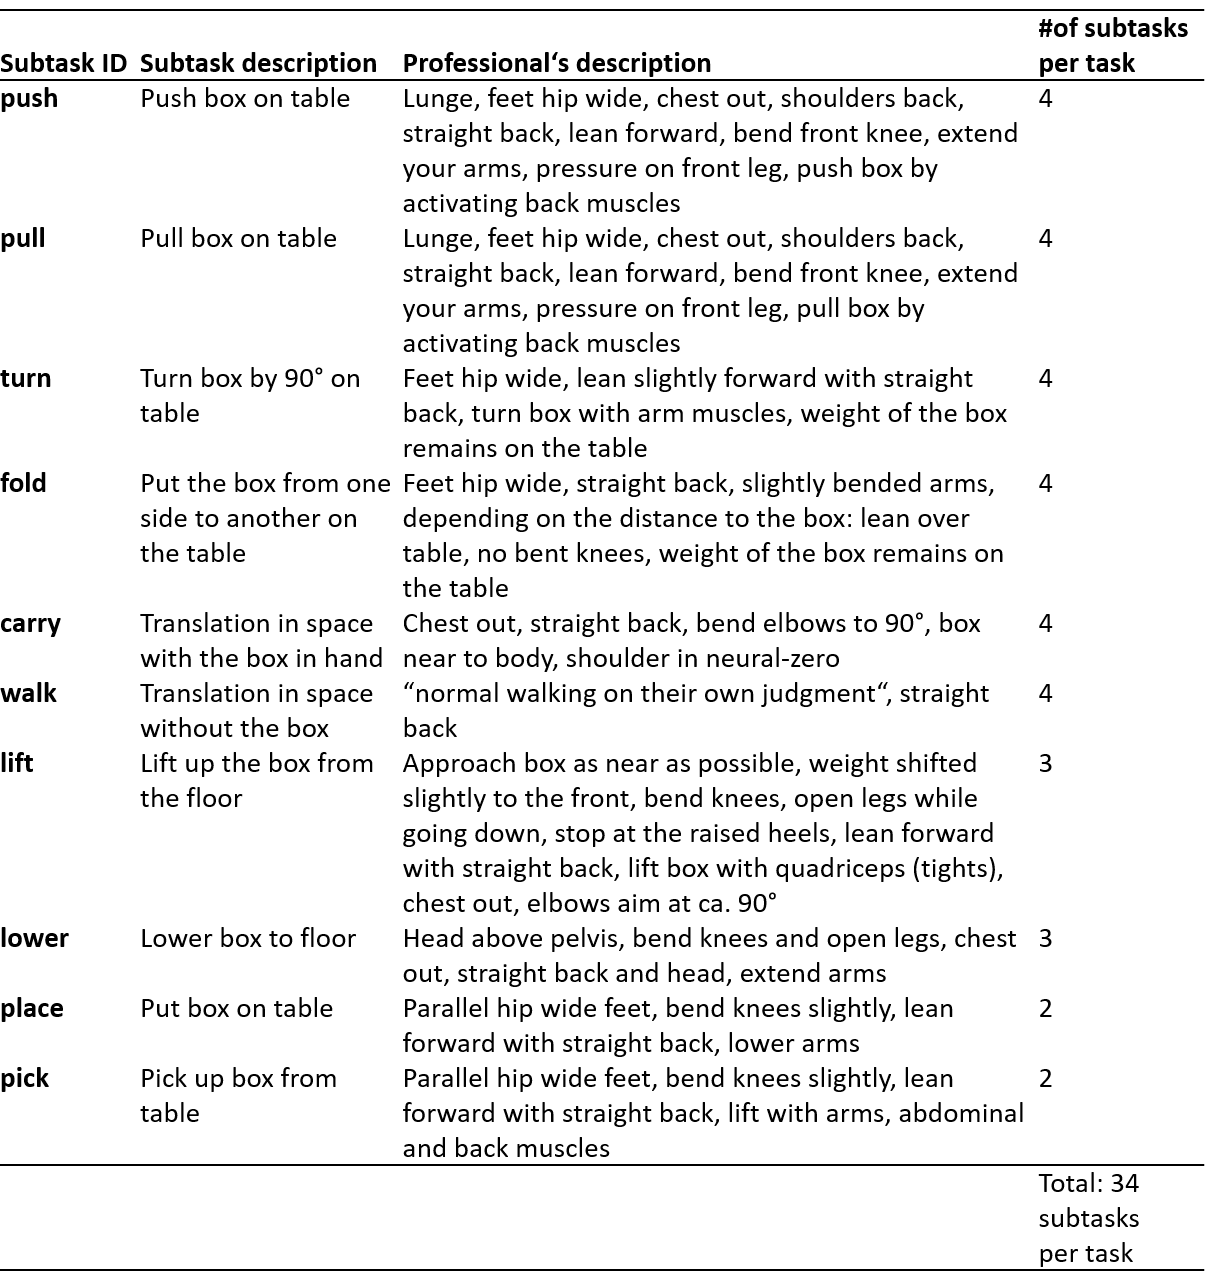
\includegraphics[width=\textwidth]{figures/sub_tasks_definition.png}
	\caption[Description of sub-tasks]{Sub-tasks that appear in every task.}
	\label{tab:sub-tasks}
\end{table}

\subsection{(c) Study Structure}
\label{sec:studyStructure}
The experiment will compare three conditions: EGO, EXO and EGO \& EXO. The main question of this section is how to assign the participants to the independent variables. The key distinction is between within-subject design and between-subject design~\cite{hornbaek}. In the within-subject design, the participant would experience all conditions. In the between-subject design, the participants would experience only one condition. Within-subject designs typically can detect the differences between the conditions more precisely (ibid.). Furthermore, within-subject designs need less participants~\footnote{The COVID-19 pandemic makes it hard to find enough participants.} than between-subject designs (ibid.). For those reasons, the study is planned to be conducted in a within-subject design.\\
However, within-subject design also has a drawback: the participants gain experience about the (i) task and the (ii) conditions during the experiment.\\

The solution for (i) is to create three tasks with nearly equal complexity. The participant will face in every condition a new task. However, the tasks are still similar, and the learning effect persists. A further reduction of the influence of the learning effect on the outcome can be countered out by counterbalancing the task.\\

(ii) implies that one condition is influenced by another condition, which the participant already experienced. Additionally, there is an asymmetrical carry-over effect between the conditions: EGO \& EXO contains condition EGO and EXO\footnote{EGO \& EXO is the union of EGO and EXO}. Thereby, EGO \& EXO influences EGO and EXO more than EGO and EXO influences EGO \& EXO. The solution to (ii) is counterbalancing, to counter the effect out.\\

Hornb\ae{}k proposes, in this case, to cross the conditions with the task and use a Greco-Latin square~\cite{hornbaek}. Three conditions and three tasks in Greco-Latin square results in blocks of nine participants. A block is depicted in figure~\ref{fig:study_session_plan}. Apart from this, Hornb\ae{}k states that experiemnts conducted within-subject should be conducted with at least 20 participants (ibid.). Because one block requires nine participants, the experiment should be conducted with at least three blocks ($3x9=27$ participants). 
The participants will have different demogaphics, which can influence the experiment's outcome, too. To reduce the demographic effect the first session of every study is for acclimatisation and is excluded from evaluation.

\begin{figure}[htb]
	\centering
	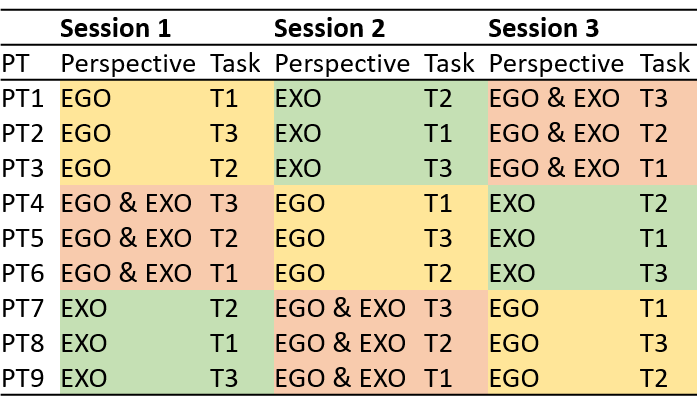
\includegraphics[width=0.5\textwidth]{figures/study_session_plan.png}
	\caption[Study structure]{Experiment structure: within-subject desing in a Greco-Latin square.}
	\label{fig:study_session_plan}
\end{figure}

\subsection{(d) Equal Task Complexity}
A study participant will face in every condition another task. For the study's validity, it is indispensable that these three tasks have nearly equal complexity. As described in (b), a task consists of 10 subtasks that occur a specific amount. The main idea to ensure a comparable complexity is to use the sub-tasks for all three tasks in an equal amount but shuffled. This means the 34 sub-tasks of task one occur in task two and three but in a different order. Table~\ref{tab:tasks} lists all three tasks. For every task, the sub-task number ST1-ST34 is provided. Every sub-task number stands for a sub-task, which comes with a description and the sub-task ID. Reading the description from top to bottom are the instructions the learner receives from the GV during one condition. The mirror mentioned in the first line is another waypoint, which is necessary for technical reasons and is described in section~\ref{sec:selfperception}.

\begin{table}[H]
	\centering
	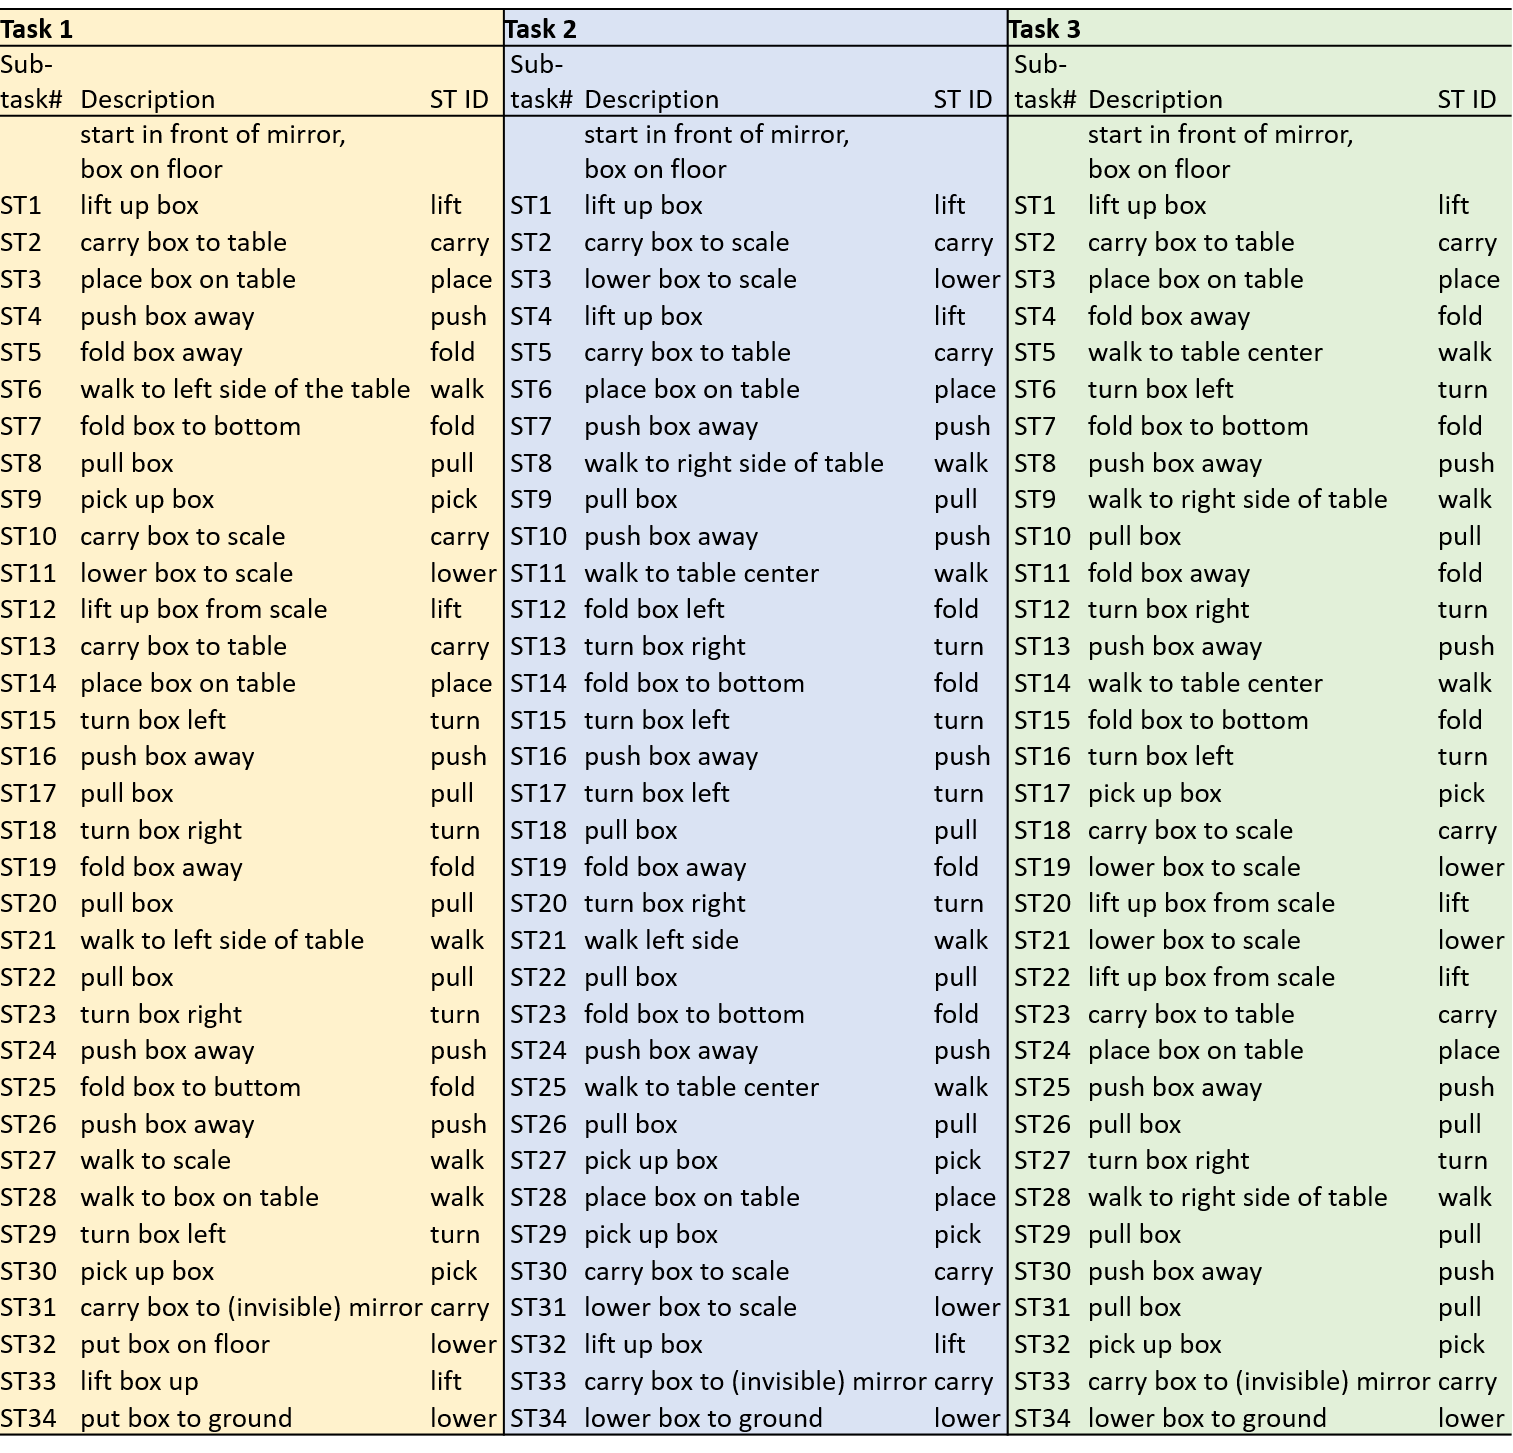
\includegraphics[width=\textwidth]{figures/tasks.png}
	\caption[Description of tasks]{tasks}
	\label{tab:tasks}
\end{table}

\section{Dependent Variables}
\label{sec:measures}
This master's thesis aims to answer the main research question RQ1: How does the visual perspective on a virtual guidance visualisation influence Motor Learning in Virtual Reality. To answer RQ1, the proposed study has to generate data that can answer the sub-research questions RQ1.1-4. This section will provide the underlying paradigm to every sub-research question and explain which measures are necessary.\\

\textbf{RQ1.1} How does the visual perspective on a virtual guidance visualisation influence movements' accuracy?\\
\textbf{Paradigma:} The more exact the learner's movements matches the GV movements, the better the learner could follow the instruction of the GV. For RQ1.1.1, the limbs of the learner and the limbs of the GV are compared. For RQ1.1.2, the box' accuracy is compared. For RQ1.1.3, both are compared and additionally, the current sub-task is taken into consideration. The accuracy can indicate how the particular movement is suited for the VP.
\begin{itemize}
	\item[] \textbf{RQ1.1.1} How does the visual perspective on a virtual guidance visualisation influence movements' accuracy of the own body?\\
	\textbf{Measures}: (1) Euclidean distance between the learners and GVs hands, feet, head and hip in meters. (2) Angle between learners and GVs the hands, feet and hip in degrees.
	
	\item[] \textbf{RQ1.1.2} How does the visual perspective on a virtual guidance visualisation influence the accuracy of handling physical load?\\
	\textbf{Measures}: (3) Euclidean distance between the learners and GVs box. (4) Angle between the learners and GVs physical load in degrees.
	
	\item[] \textbf{RQ1.1.3}How does the visual perspective on a virtual guidance visualisation influence sub-tasks accuracy?\\
	\textbf{Measures}: (1-4), additionally matched to the sub-tasks that is currently performed (5).
\end{itemize}	
(1-4) gives insights to what extend the learner could follow the GV for the whole task. (5) can extract specific sub-tasks for which the learner could follow the GV to a certain extend. For example, in the ego-centric VP, the overall accuracy for a task is lower than in the other VPs, but the accuracy for the sub-tasks \textit{lift} and \textit{lower} is higher than in other VP. For this example, measure (5) can extract specific sub-tasks that are performed better or worse than in other VPs.\\

\textbf{RQ1.2} Does the visual perspective on a virtual guidance visualisation influence the transfer of ergonomic principles?\\
\textbf{Paradigma:} the more exact the learner's RM matches the GVs RM, the better the ergonomic principles could be transferred.\\
\textbf{Measures:} (6) Risk Measurements: (6.1) \textit{upright stance} in degrees, (6.2) \textit{squat} in meters, (6.3) \textit{good base} in meters, (6.4) box-near-body in meters.\\

\begin{itemize}
	\item[] (6.1) \textit{upright stance} is defined by the difference in degrees between the straight upward vector and the back of the learner. For all sub-task, \textit{upright stance} should be in a certain window, see~\ref{sec:ergonomicMeasurements}. Upright stance indicates if the learner could percept the correct posture of his back.
	
	\item[] (6.2) \textit{squat} is defined by the distance in meters between the feet. For the sub-tasks \textit{lift} and \textit{lower}, the squat distance should be in a specific window. For the other sub-tasks, \textit{squat} is not applied because the knees do not bend in the other sub-tasks. \textit{Squat} indicates if the learner could percept that he should bend his knees during \textit{lift} and \textit{lower}.
	
	\item[] (6.3) \textit{good base} is defined by the distance in meters between the feet. For the sub-tasks \textit{push}, \textit{pull}, \textit{turn}, \textit{fold}, \textit{lift}, \textit{lower}, \textit{pick} and \textit{place}, \textit{good base} should be in a specific window. Good base indicates if the learner could percept the correct posture of the feet.
	Muckell et al.\cite{muckell} additionally use the RM \textit{spine twist} in their work. This RM cannot be applied for this experiment because of the multiple-represention mechanic. The learner has multiple GV around and is free of choice which one to look at. The turn of the head implies spine twist. Though, \textit{spine twist} would have a low validity and reliability.
	
	\item[] (6.4) box-near-body. During the task design, a professional physiologist was consulted. During the interview, all movements were described in detail, compare table~\ref{tab:sub-tasks}. During the sub-task \textit{carry}, the box should be as near as possible to the body, while the elbows should have a bend angle of 90 degrees. The physiologist stated this posture as important. This statement is the basis to introduce a additional risk metric related measurement: box-near-body. Unfortunately, the bend angle could not be determined during a study for technical reasons, see chapter~\ref{chapter:system}. Fortunately, the distance between box and hip can be determined. Box-near-body is defined as the distance in meters between the learner's box and hip. For the sub-task \textit{carry}, box-near-body should be in a certain window.
\end{itemize}

RM (6.1-4) are different from accuracy measurements (1-5) because they are independent of the learner's position and the GVs position. For example, in the exo-centric VP, a learner cannot percept the correct position where he/she should stand. The learner thereby stands 15cm away from the position he/she should stand. The overall accuracy is thereby lower. But the learner could percept the positioning of his/her feet correctly. In this case, the RM (6.3) are fulfiled while the accuracy is biased.\\

\textbf{RQ1.3} How does the visual perspective on a virtual guidance visualisation influence the learner's visual focus?\\
Measures: (7) \textit{looking at}\\
Paradigma: the learner's visual focus is on the object the learner is looking at.\\
The learner interacts with a box and has multiple GVs around and inside the learner. \textit{Looking at} can give insights on which GV the learner is focusing, the frequency of focus changes and the role of the physical load.

\textbf{RQ1.4} What is the subjective personal preference of the learner for the visual perspectives?\\
Measures: (8) qualitative data; Likert scales, semi-structured interview, digging into incidences. After each session, a "after session questionaire" is handed to the participant. After all three sessions, a semi-structured interview is conducted.\\
The qualitative data serves not only to investigate the learner's personal preference but also to serve as triangulation method for (1-7).\\

The last measure is the (9) task completion time (TCT) measured in milliseconds. The speed-mechanic regulates the speed of the animation of the GV. The further the learner is located to the GV, the slower the GV animation speed until it stops entirely at $EDT_{max}$. The task completion time can give insights into what extent the learner could perceive the desired position of his/her body in relation to the GV. This measure relates to (1) and can be used for triangulation.
Additionally, it is to expect that the TCT is decreasing from condition to condition because the participant acclimated. By that, TCT could give insights into the learning effect between the conditions. Finally, the study is recorded by video. If during the evaluation arises questions about a specific topic, the recordings can be consulted.

